\begin{figure*}[t]
\centering
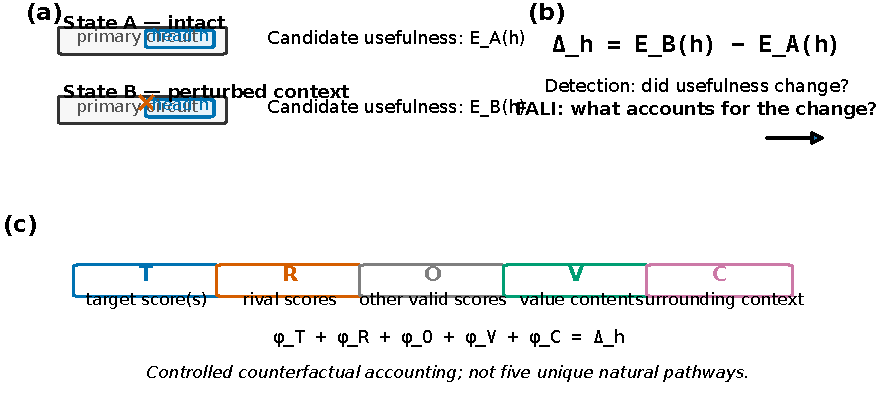
\includegraphics[width=\textwidth]{figures/Fig1.pdf}
\caption{\textbf{FALI resolves a conditional change in a selected attention head's causal usefulness.}
(a) The same candidate head $h$ is evaluated in an intact state $A$ and a prespecified perturbed state $B$.
(b) The quantity to be explained is the cross-state change $\Delta_h=E_B(h)-E_A(h)$ in output-grounded causal usefulness.
(c) FALI attributes this endpoint change under an explicit intervention game across task-target scores ($T$), rival scores ($R$), other structurally valid scores ($O$), value content ($V$), and surrounding-network context ($C$), with Owen efficiency $\phi_T+\phi_R+\phi_O+\phi_V+\phi_C=\Delta_h$.
The candidate head and task-relevant target coordinates are specified before FALI analysis.}
\label{fig:fali-overview}
\end{figure*}
